\graphicspath{{figures/appendix/}}
\chapter{Test Journal: Gear Train System}\label{appendix:DCMotorInductance}
\begin{table}[htbp]
\begin{tabular}{l l}
\textbf{Test participants:} & Maxime \& Geoffroy  \\
\textbf{Date:}  & 28/2-2017
\end{tabular}
\end{table}

\section*{Purpose}
The objective of this test is to determine all the of the gear train system composed of the DC motor and the gear train.
\section*{Electronics characteristics}

\subsection{Internal Inductance of the DC Motor $L_a$}
\begin{table}[htbp]
	\centering
	\caption{List of measurement equipment and components}\label{tab_appendix:LaSetUp}

	\begin{tabularx}{\textwidth}{lXXXX}
		Name 				& Brand	& Model & AAU-number									\\ \toprule \rowcolor{lightGrey}
		Oscilloscope	& Agilent & 54621D & 33941 	\\
		Powersupply	& Agilent & E3631A & 78577\\ \rowcolor{lightGrey}
		DC motor & Alsthom BBC & F9M2& 08339
	\end{tabularx}
\end{table}
\subsubsection*{Setup}
\autoref{fig:LaMeasurementSetup} shows a diagram and photo of the measurement set up
\begin{figure}[htbp]
	\centering
	\begin{subfigure}{0.50\textwidth}
		\includegraphics[width=0.5\textwidth]{MotorImpedanceTest.jpg}
		\caption{Diagram of the setup.} \label{fig:LaMeasurementDiagram}
	\end{subfigure}
	\begin{subfigure}{0.40\textwidth}
		\includegraphics[width=1\textwidth]{MotorImpedanceTest.jpg}
		\caption{Picture of the setup.} \label{fig:LaMeasurementPictures}
	\end{subfigure}
	\caption{The measurement setup.} \label{fig:LaMeasurementSetup}   
\end{figure}

\subsubsection*{Method}
This test consists of having the motor shaft locked while a step is applied. The voltage of a shunt resistor is then measured by an oscilloscope from which the current is deduced.
\subsubsection*{Raw data}
\autoref{fig:LaTestCurrentPlot} is plot of the evolution the current of the circuit in respect to time.

\begin{figure}[htbp]
	\centering
	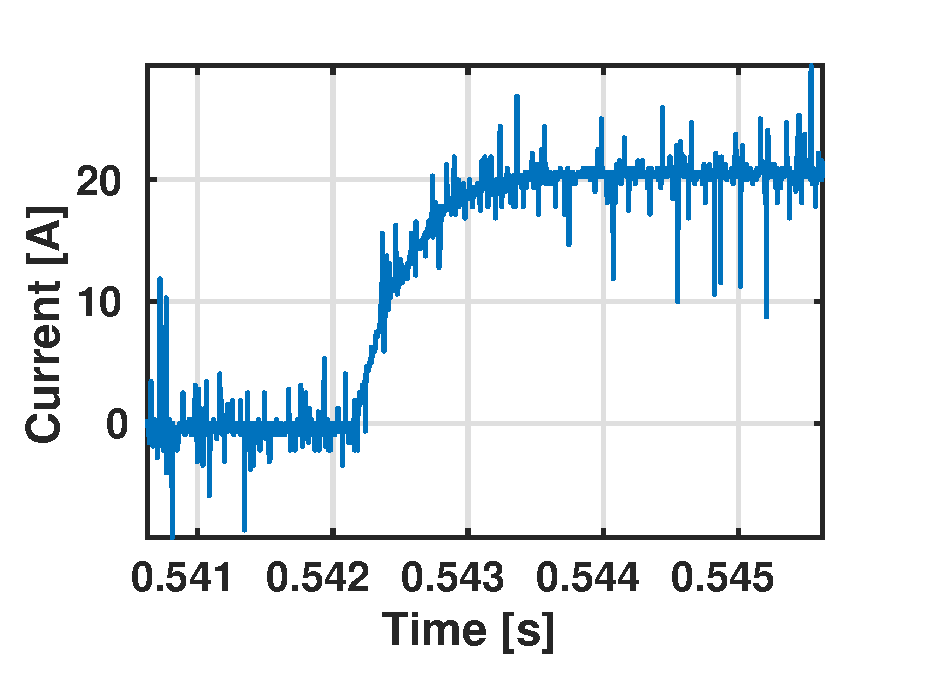
\includegraphics[width=0.7\textwidth]{LaTestCurrentPlot}
	\caption{Plot of the current in respect to time}\label{fig:LaTestCurrentPlot}
\end{figure}

\subsubsection*{Data processing}
When the shaft is locked and a step is applied the DC motor's electric equation can be resumed as in \autoref{eq:LaEquation}.
\begin{equation}
	F(s)=\frac{I_a(s)}{U_a(s)}=\frac{\frac{1}{R_a}}{\frac{L_a}{R_a} s+1} \addunit{1}
	\label{eq:LaEquation}
\end{equation}
\startexplain
\explain{$I_a(s)$ is the current in Laplace domain}{1}
\explain{$U_a(s)$ is the body's acceleration}{1}
\explain{$R_a$ is the internal resistance of the motor}{\si{\ohm}}
\explain{$L_a$ is the internal inductance of the motor}{\si{\henry}}
\stopexplain

When a unit step response is applied to the system \autoref{eq:LaEquation} becomes \autoref{eq:LaEquationStep}.

\begin{equation}
F(s)=\frac{\frac{1}{R_a}}{\frac{L_a}{R_a} s+1}\frac{1}{s}=\frac{-\frac{1}{R_a}}{s+\frac{R_a}{L_a}}+\frac{1}{R_a s} \addunit{1}
\label{eq:LaEquationStep}
\end{equation}

\autoref{eq:LaEquationStep} is then put in the continuous time domain to get \autoref{eq:LaEquationStepTime}.

\begin{equation}
f(t)= \frac{1}{R_a} \left(1-e^{-\frac{R_a}{L_a} t}\right) \addunit{1}
\label{eq:LaEquationStepTime}
\end{equation}

\autoref{eq:LaEquationStepTime} means that at $t=\frac{L_a}{R_a}$ the function would give $1-e^{-1}=\SI{63.212055882}{\percent}$ of its settling value. So at \SI{63.212055882}{\percent} of the settling value $t=\frac{L_a}{R_a}$ and since $R_a=\SI{0.43}{\ohm}$ \cite{datasheet:saradc} is known finding $L_a$ becomes trivial.

\subsubsection*{Conclusion}

Since the value of the current at the settling value is \SI{20.471}{\ampere}. Then \autoref{eq:LaEq} gives the value of $L_a$.

\begin{subequations} \label{eq:LaEq}
	\begin{flalign}
		&\frac{1}{R_a} \left(1-e^{-\frac{R_a}{L_a} \tau}\right)=20.471 \cdot 0.63212055882 \addunit{\second} \\
		&t = \SI{0.00190}{\second} \\
		&L_a=tR_a \\
		&L_a=\SI{817}{\micro\henry}
	\end{flalign}
\end{subequations}

\subsection{Internal Resistance of the DC Motor $R_a$}

\subsection{The DC Motor velocity constant $K_e$}

\begin{table}[htbp]
	\centering
	\caption{List of measurement equipment and components}\label{tab_appendix:KeSetUp}
	
	\begin{tabularx}{\textwidth}{lXXXX}
		Name 				& Brand	& Model & AAU-number									\\ \toprule \rowcolor{lightGrey}
		Oscilloscope	& Agilent & 54621D & 33941 	\\
		Powersupply	& Agilent & E3631A & 78577\\ \rowcolor{lightGrey}
		DC motor & Alsthom BBC & F9M2& 08339
	\end{tabularx}
\end{table}

\subsubsection*{Setup}
\autoref{fig:KeMeasurementSetup} shows a diagram and photo of the measurement set up
\begin{figure}[htbp]
	\centering
	\begin{subfigure}{0.50\textwidth}
		%\includegraphics[width=0.5\textwidth]{}
		\missingfigure{Diagram of the setup}
		\caption{Diagram of the setup.} \label{fig:KeMeasurementDiagram}
	\end{subfigure}
	\begin{subfigure}{0.40\textwidth}
		%\includegraphics[width=1\textwidth]{MotorImpedanceTest.jpg}
		\missingfigure{Picture of the setup}
		\caption{Picture of the setup.} \label{fig:KeMeasurementPictures}
	\end{subfigure}
	\caption{The measurement setup.} \label{fig:KeMeasurementSetup}   
\end{figure}

\subsubsection*{Method}
This test consists of having the motor shaft in steady state while the voltage $U$ of the generator, the angular velocity $\omega$ of the shaft and the current $I$.

\subsubsection*{Raw data}
\autoref{tab:KeTest} has all the measurements done.


\subsubsection*{Data processing}

When the shaft is rotating in steady state as shown in \autoref{fig:KeMeasurementDiagram}, \autoref{eq:KeSetUpElec} can be derived.
\begin{equation}
U=K_e\omega+R_m I \addunit{V}
\label{eq:KeSetUpElec}
\end{equation}
\startexplain
\explain{$I$ is the current in the circuit}{\si{\ampere}}
\explain{$U$ is the generator's voltage}{\si{\volt}}
\explain{$K_e$ is the velocity constant of the motor}{\si{\volt\per\radian\second}}
\explain{$R_m$ is the internal resistance of the motor}{\si{\ohm}}
\stopexplain

From \autoref{eq:KeSetUpElec} \autoref{eq:KeForm} is obtained by isolating $K_e$.

\begin{equation}
K_e=\frac{U-R_m I}{\omega} \addunit{\volt\per\radian\second}
\label{eq:KeForm}
\end{equation}

explain first results are bad so only takes last ones then use average.

\subsubsection*{Conclusion}

compare Ke to mesured with something so can say it is okay

\subsection{The DC Motor torque constant $K_t$}


\section{Mechanical Characteristics}
\subsection{Frictions $B_a$}

\subsection{Moment of Inertia $J_a$}
